% TODO (but maybe not here?): explain why and how we define our own meta schema based on json schema, because we use just subset of its features and because our schema is used to generate schema editor GUI and therefore should only show what is supported. Also we want to add descriptions and maybe more. Also limit options to not overwhelm and confuse the user.
% TODO also describe more the users perspective how users would use the tool?

% felix
\subsection{User Interface}\label{subsec:overview}
The design of \toolname{} is strongly inspired by another tool by one of the authors, which is a configurator GUI for the Minecraft server plugin BossShopPro\cite{bossshoppro}, where the GUI components are generated based on a rudimentary custom schema language and several inbuilt schemas.
That tool provides the user a text editor panel for editing configuration files of that domain in a text editor, as well as a GUI editor panel, where the user can edit their configuration file using GUI components.\cite{githubBspEditor}
\toolname{} differs from that tool by being generic, instead of being bound to a certain domain, by having a much more expressive schema language, a schema editor and many other features that improve the user experience, such as a search functionality.
%TODO: maybe move to related work?

Before we dive into the architecture and detailed design of the tool, this section provides an overview of the tool from the view of the user.

The user interface has three distinct views:
\begin{enumerate}
	\item File Editor (figure \ref{fig:fileeditor}): In this view the user can modify their \cfgfile{}, based on a schema.
	\item Schema Editor (figure \ref{fig:schemaeditor}): In this view the user can modify their schema.
	\item Settings (figure \ref{fig:settings} in appendix): In this view the user can adjust parameters of the tool.
\end{enumerate}


Figures \ref{mockup_gui_config} and \ref{mockup_gui_schema} (appendix) provide a sketch of the planned user interface design before the implementation.


\begin{figure*}
    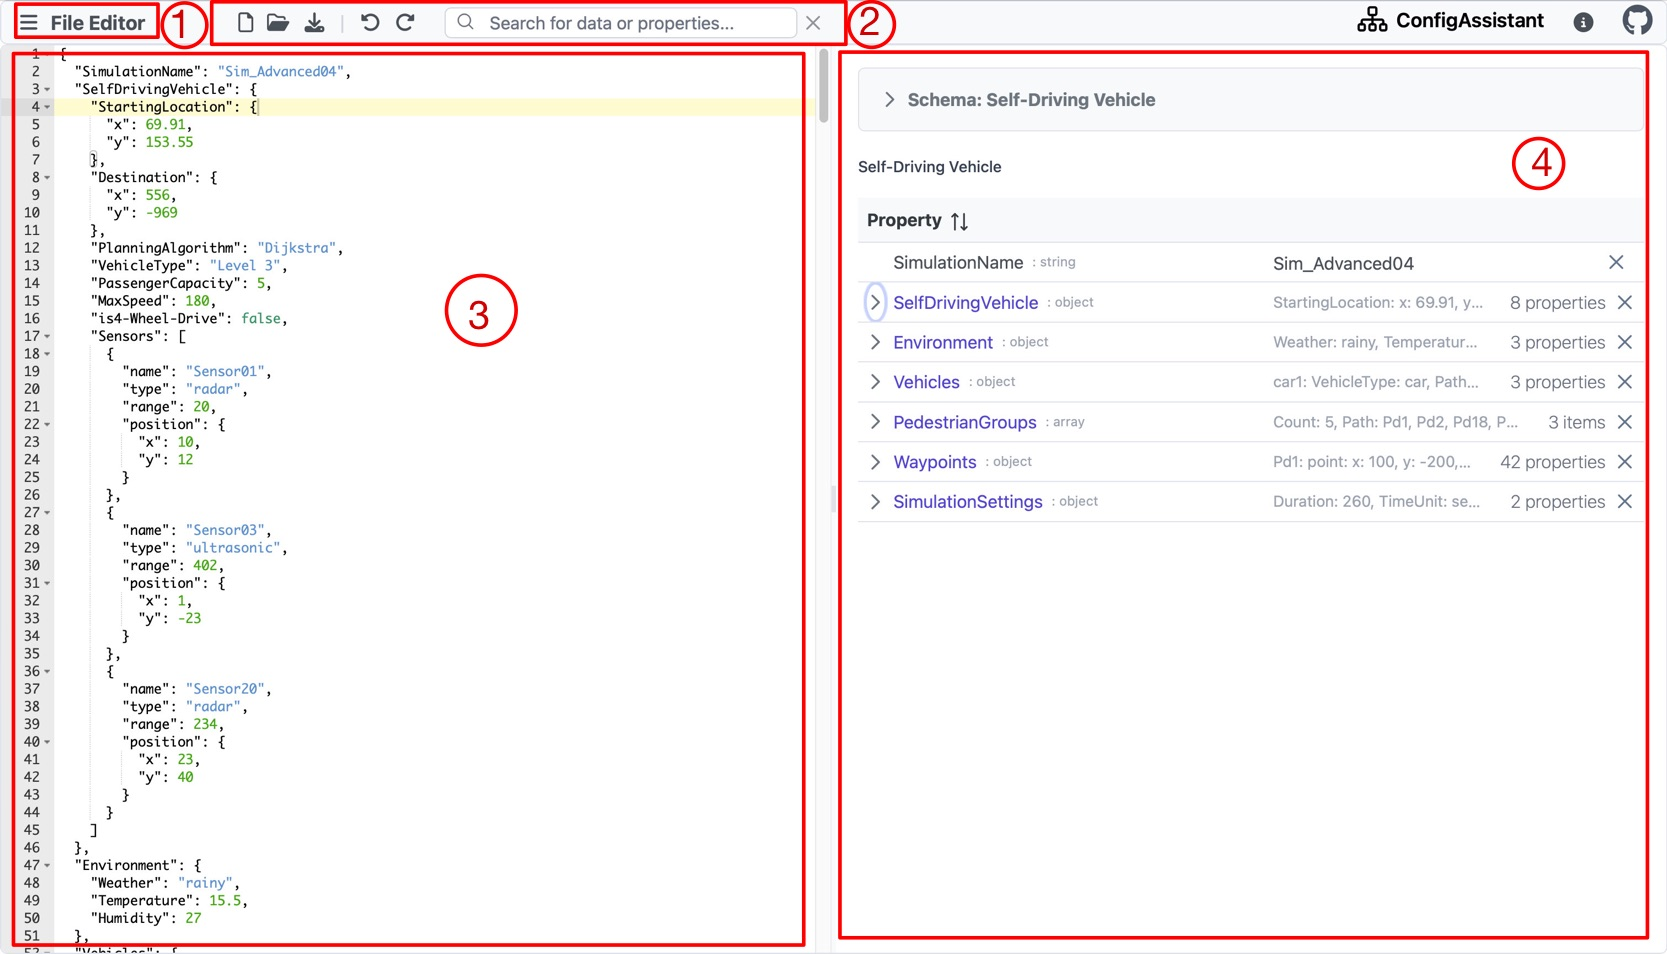
\includegraphics[width=\textwidth]{figures/fileeditor}
    \caption{UI of File Editor view. Different components highlighted in red: 1) button to switch to other view (e.g. to Schema Editor view), 2) Toolbar with various functionality, 3) Code panel, 4) GUI panel}
    \label{fig:fileeditor}
\end{figure*}

\begin{figure*}
    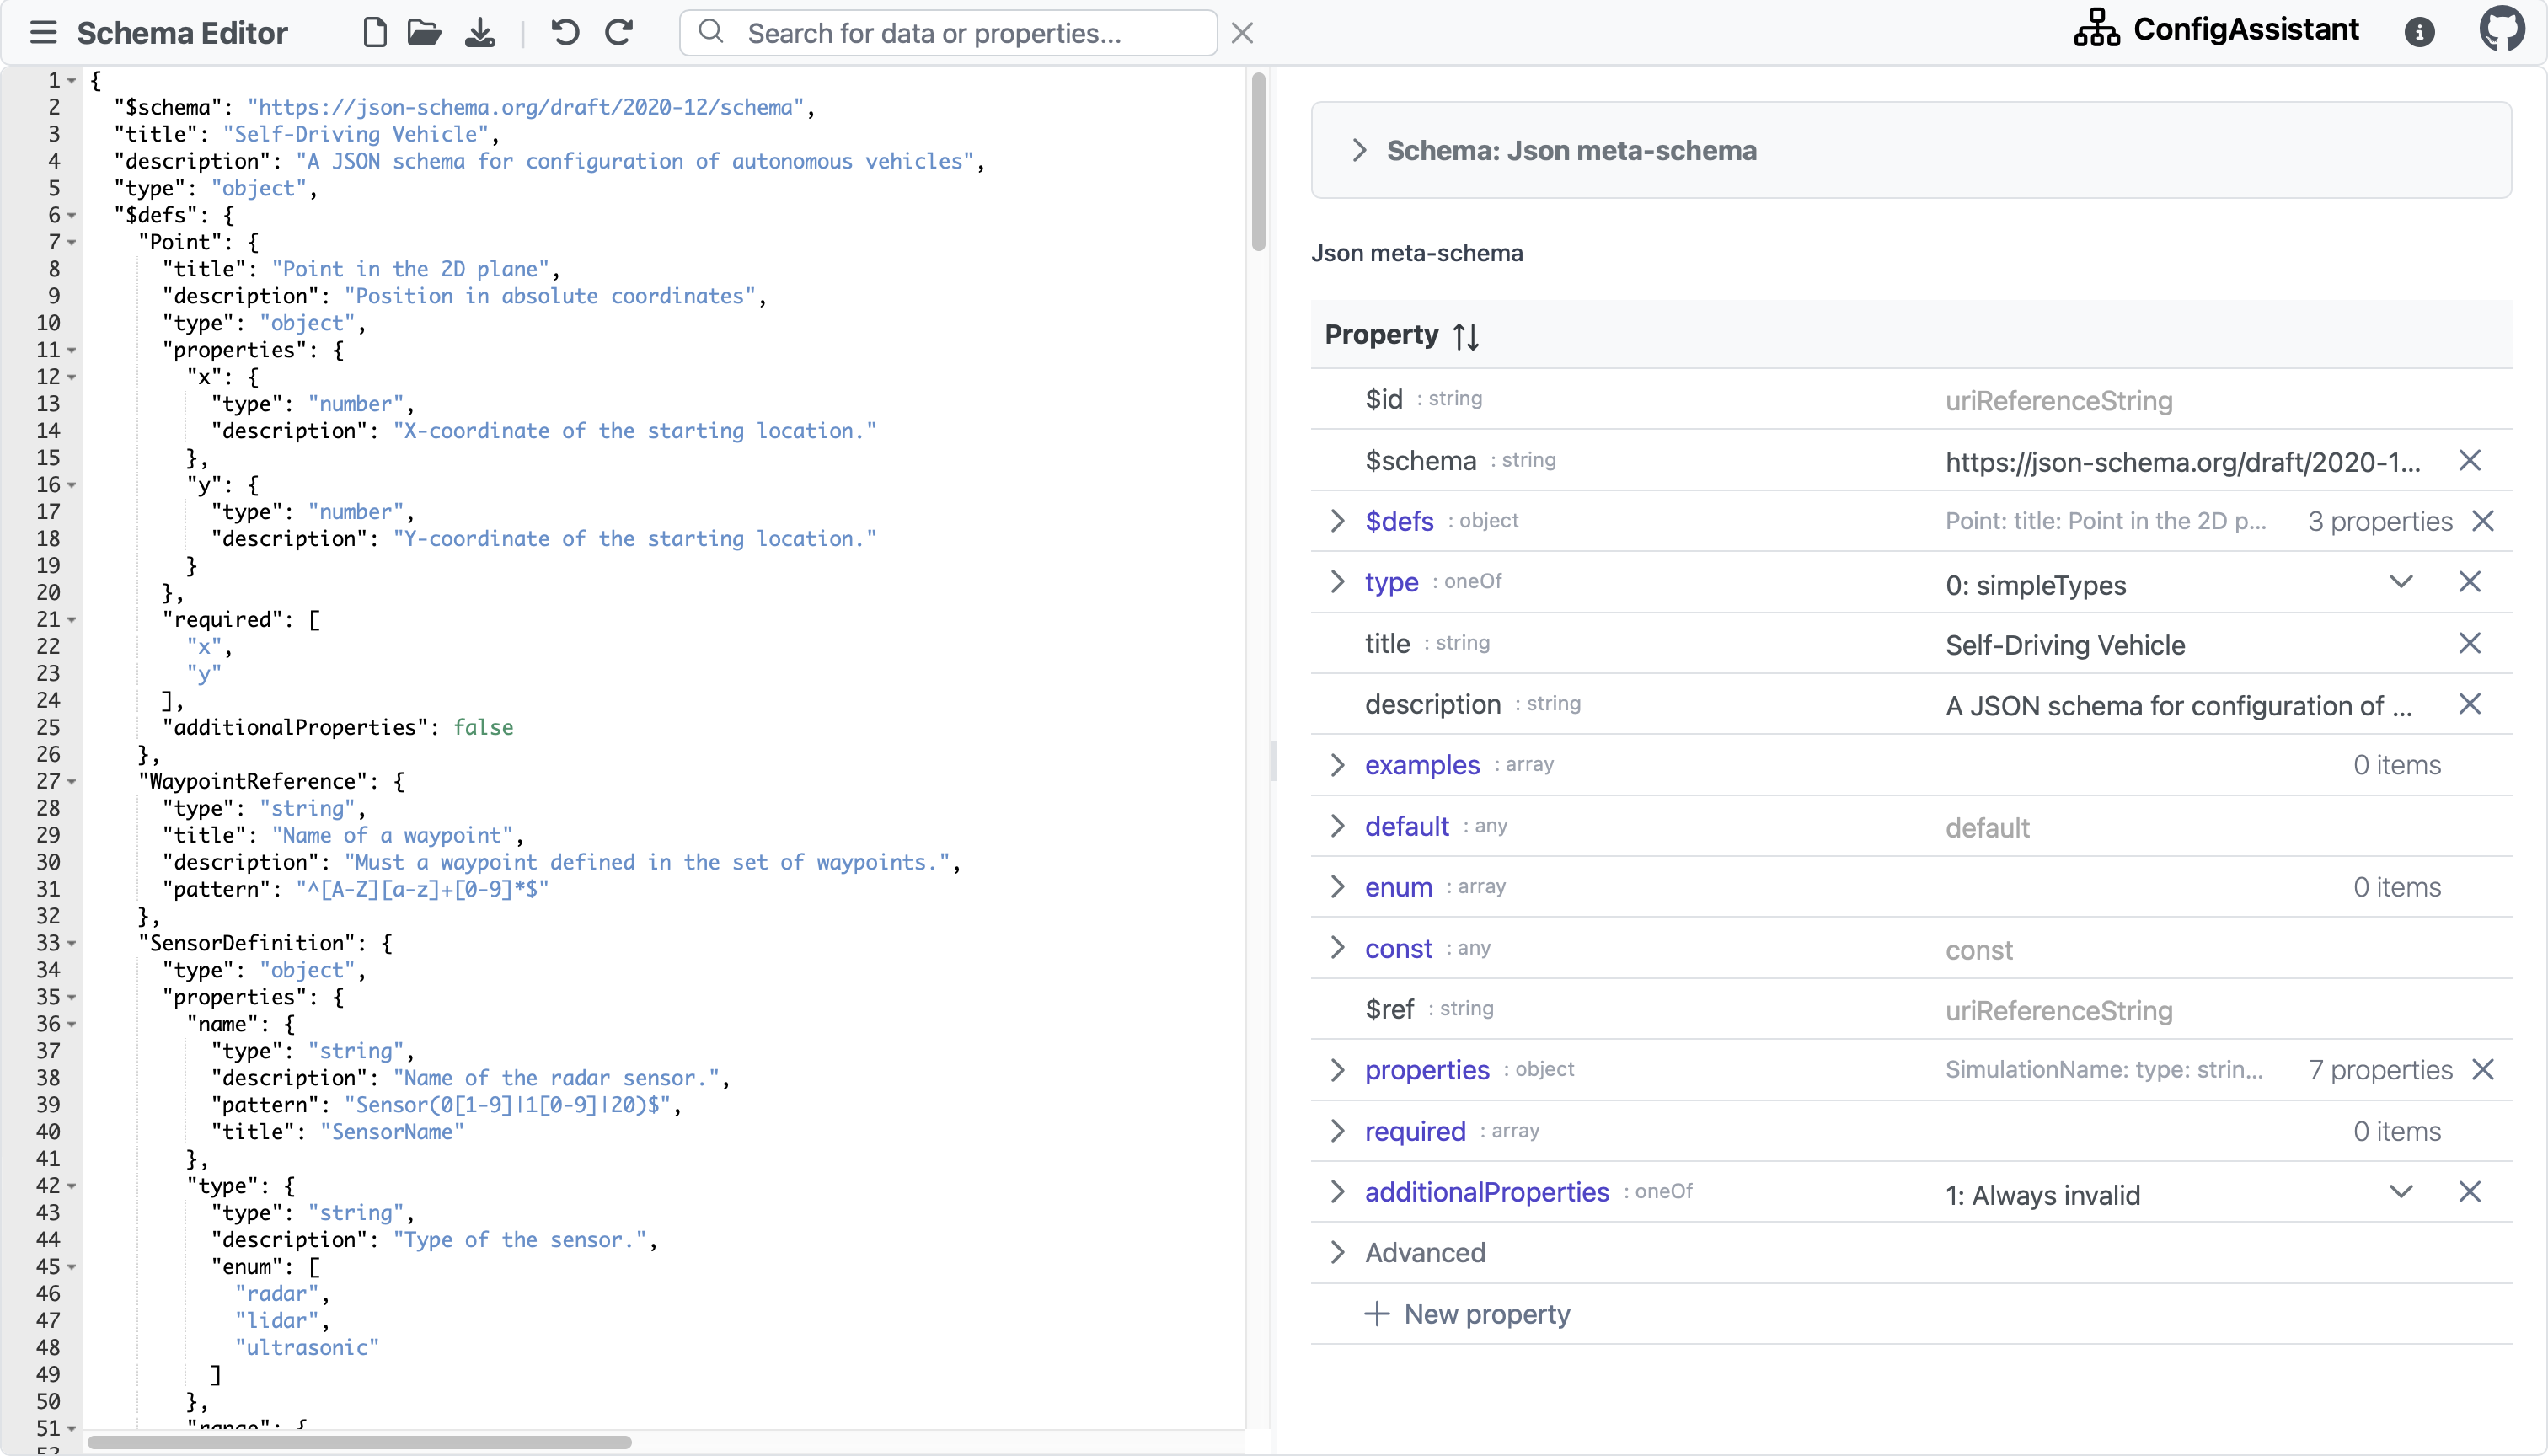
\includegraphics[width=\textwidth]{figures/schemaeditor}
    \caption{UI of Schema Editor view}
    \label{fig:schemaeditor}
\end{figure*}


The UI is divided into two main panels: the  \textit{Code panel} (on the left) and the \textit{GUI panel} (on the right).
In the \textit{Code panel} the user can modify their data by hand, as in a regular code editor.
Features, such as syntax highlighting and schema validation, assist the user.
In the \textit{GUI panel}, the user can modify their data with the help of a GUI.
The GUI is based on the schema which the user provides (more on that in the next paragraphs).
For example, for enum properties, the user will get a dropdown menu with the different options to choose from and for boolean properties the user will get a checkbox.
Other features, such as tooltips that display the description and constraints of a property, further assist the user.

This design combines the benefits of both a rich text code editor (efficient for many tasks, more suited for users with technical understanding of the data structure) with the benefits of a GUI (enables users without deep technical understanding to work with the data, assists also expert users).

As a schema is a \cfgfile{} itself, it can be treated as such and the tool can offer assistance accordingly.
Note that whenever the user edits a \cfgfile{} using the tool, they do so using some underlying schema.
Even the tool settings can be seen as a \cfgfile{}, for which the underlying schema is a settings schema.

Table \ref{tab:schema_and_file_data_by_mode} illustrates how for the different views, file data and schema being used by the tool differ.
\begin{table}[!t]
\caption{File data and schema for the different views}
\label{tab:schema_and_file_data_by_mode}
\centering
\begin{tabular}{lll}
\toprule
\textbf{View} & \textbf{Effective File Data} & \textbf{Effective Schema} \\
\midrule
File editor   & User data                    & User schema               \\
Schema editor & User schema                  & JSON Meta Schema          \\
Settings      & Settings data                & Settings schema           \\
\bottomrule
\end{tabular}
\end{table}


\subsection{Intended Workflow}\label{subsec:workflow} %keyuri
\begin{enumerate}
    \item Upon initial access of \toolname{}, a dialog is displayed, where users can select their desired schema.
    \item After selecting a schema, the user will find that a GUI is automatically generated on the right-hand side of the File Editor,
    tailored to the selected schema.
    \item Through the GUI panel, users are assisted in creating or modifying \cfgfiles{}.
    \item If a user wishes to modify the selected schema, such as adding new properties, they can do so through the schema editor.
    Changes can be made using either the GUI panel or the code panel, and these modifications will automatically reflect in the file editor.
\end{enumerate}

%\begin{figure}[!htb]
%    \begin{minipage}[t]{0.5\textwidth}
%        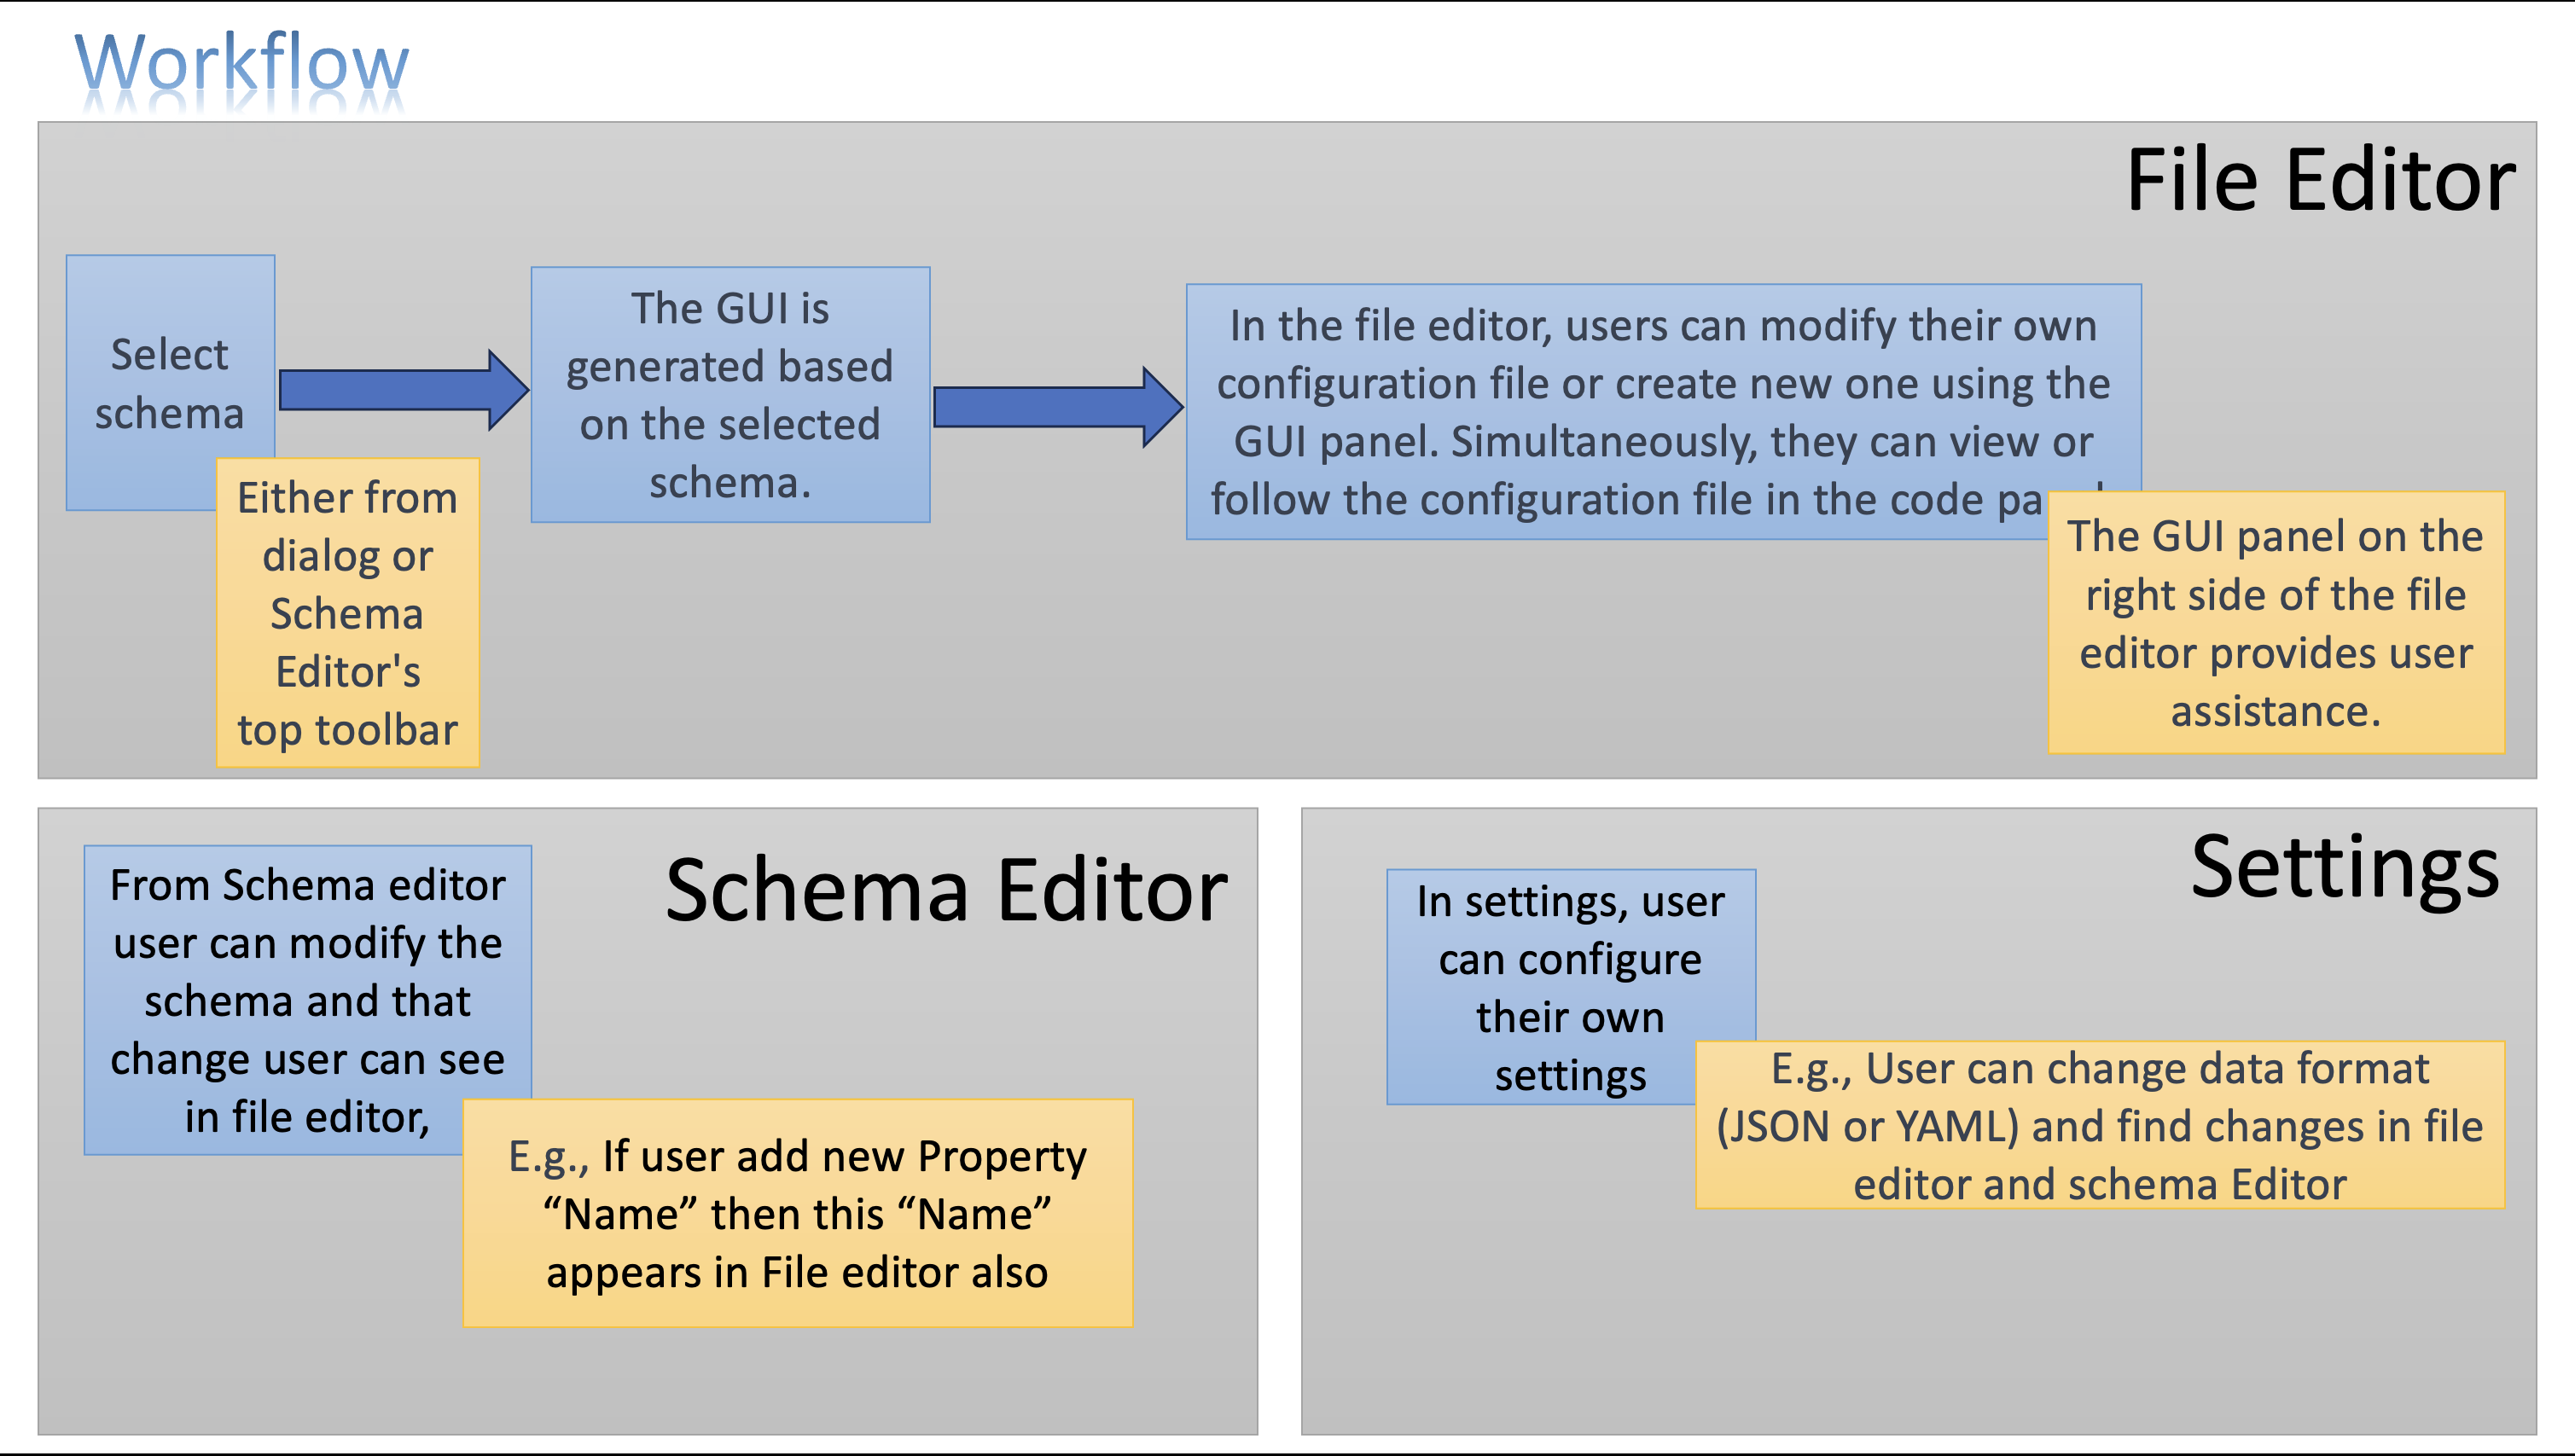
\includegraphics[width=3.5in]{figures/Toolworkflow}
%        \caption{Workflow}
%        \label{workflow}
%    \end{minipage}\label{fig:workflow}
%\end{figure}




% felix

\subsection{Architecture}\label{subsec:architecture} % todo diagram illustrating the architecture
This section describes our main architectural design decisions.
Those will not be relevant or visible for the user of the tool, but are important for understanding our implementation.
Aim of those design decisions is to ensure modularity and maintainability of the tool.

The core of \toolname{} is a single source of truth data store that contains the current user configuration data (as a JavaScript Object).
With this data store we can bidirectionally connect what we call ``editor panels''.
An editor panel is a modular component that the user of the tool can access to modify the config data in an indirect way.
It might be implemented as a code editor, a graphical user interface or any other way in which the data can be presented to the user.
All editor panels are independent and do only have access to the data store but not to each other.
Every editor panel subscribes to the changes of the data store, so it can be updated accordingly whenever the data in the store is changed.
Additionally, every panel has the capabilities of updating the data store themselves, which is done when the user modifies the data in the editor panel.
The following artificial example use-cases illustrate the capabilities of this architecture:

\begin{itemize}
    \item Format converter: one panel shows the data in a code editor in JSON format, a second panel shows the data in a code editor in YAML format. Any semantic data change on one panel will cause the same semantic change in the other panel.
    \item Split-Screen Editor: one panel shows the data in a code editor, a second panel shows the data in a GUI. This way the user can have the efficiency of a text editor, but also the assistance of a GUI at the same time. Any semantic data change on one panel will be forwarded to the other panel.
    \item The Split-Screen Editor could be implemented for different data formats, such as YAML, JSON and XML. The architecture allows any data format as long as there exists a mapping from this data format to a JavaScript Object and back.
\end{itemize}

In practice, we implement only one code editor panel, as well as one GUI editor panel. 
The architecture, however, would be flexible enough to allow replacing any of these panels or adding new ones, since they are decoupled from each other and only communicate with the single source of truth data store.

% TODO: Add diagram with store in center in several panels with bidirectional connection of subscribe/update

% felix

\subsubsection{Single Source of Truth Data Store}
This is the core of the tool.
The panels can subscribe to this store to receive updates whenever data is changed.
Also, panels can trigger changes of the data in the store.
Besides the current configuration data, the store also stores the path of the currently selected data entry and the schema that is currently being used.

% felix

\subsubsection{Code Panel}\label{subsubsec:design_text_editor_panel} 
For the code panel, we embed a rich-text code editor that already supports syntax highlighting and other useful features.
We enable validation of whether the text is well-formed according to the JSON/YAML/XML Standard and add schema validation.
The panel subscribes to the data store.
Whenever the configuration data is changed in the store, the panel will take the new configuration data JavaScript Object, serialize it into the given data format and replace the text in the code editor with the new serialized data.
The action of replacing the text in the code editor will cause formatting and comments to be lost, which we accept.
In the future, several mechanism could be applied to avoid the loss of formatting or comments (see section \ref{subsec:future-work}).

When the user edits the text in the code editor, the text is deserialized into a JavaScript Object and sent to the data store, which then updates the configuration data object and notifies all other subscribed panels of the change.


To enable communication with the store, for any data format that the tool should support, we need a function to stringify a JavaScript object to a string in the data format and a function to parse a string in that data format as a JavaScript object.


To make it possible to highlight certain lines in the editor as erroneous (schema violations) or jump to certain lines (e.g. when the user selects a property in the GUI editor, we want to jump to the same property in the text editor), we need a function \texttt{determineRow(editorContent, dataPath)} that can determine the corresponding editor line, based on the configuration text and a given data path. 

The other way around, when the user places their cursor inside the text editor, we want to determine the path of the element that the cursor is currently at. This requires a function \texttt{determinePath(editorContent, cursorPosition)} which returns a data path based on the configuration text and a given cursor position.

% felix

\subsubsection{GUI Assistance Panel}
The GUI assistance panel directly works with the given schema and provides the user with corresponding GUI elements, such as a checkbox for a boolean data structure or a text field for a string data structure.
Additional GUI elements, such as tooltips (showing the description of a data field) are used to support the easier.
The GUI elements are constructed in the following manner: a schema is seen as a hierarchical tree of data field definitions and their corresponding constraints.
A data field can either be simple (string, boolean, number, integer) or complex (array or object with children).
Every schema has a root data field.
The GUI element for this root data field is constructed.
When constructing the GUI element for a complex data field, all GUI elements of the child data fields are constructed too, in a recursive manner.
This way, the whole schema tree is traversed and GUI elements for all entries are constructed.
To avoid overwhelming the user with too many GUI elements, the ones with child elements can be expanded or collapsed by the user and only a limited amount of them is expanded by default.
By design, each of these constructed GUI elements is mapped to their corresponding data field (in other words: to a path in the data structure).
The initial values of all GUI elements are taken from the data in the store, by accessing the data at the given paths.
Whenever the values in a GUI element are adjusted by the user, the data in the store will be updated with the new values.


